% Options for packages loaded elsewhere
\PassOptionsToPackage{unicode}{hyperref}
\PassOptionsToPackage{hyphens}{url}
\PassOptionsToPackage{dvipsnames,svgnames,x11names}{xcolor}
%
\documentclass[
  number]{elsarticle}

\usepackage{amsmath,amssymb}
\usepackage{iftex}
\ifPDFTeX
  \usepackage[T1]{fontenc}
  \usepackage[utf8]{inputenc}
  \usepackage{textcomp} % provide euro and other symbols
\else % if luatex or xetex
  \usepackage{unicode-math}
  \defaultfontfeatures{Scale=MatchLowercase}
  \defaultfontfeatures[\rmfamily]{Ligatures=TeX,Scale=1}
\fi
\usepackage{lmodern}
\ifPDFTeX\else  
    % xetex/luatex font selection
\fi
% Use upquote if available, for straight quotes in verbatim environments
\IfFileExists{upquote.sty}{\usepackage{upquote}}{}
\IfFileExists{microtype.sty}{% use microtype if available
  \usepackage[]{microtype}
  \UseMicrotypeSet[protrusion]{basicmath} % disable protrusion for tt fonts
}{}
\makeatletter
\@ifundefined{KOMAClassName}{% if non-KOMA class
  \IfFileExists{parskip.sty}{%
    \usepackage{parskip}
  }{% else
    \setlength{\parindent}{0pt}
    \setlength{\parskip}{6pt plus 2pt minus 1pt}}
}{% if KOMA class
  \KOMAoptions{parskip=half}}
\makeatother
\usepackage{xcolor}
\setlength{\emergencystretch}{3em} % prevent overfull lines
\setcounter{secnumdepth}{5}
% Make \paragraph and \subparagraph free-standing
\ifx\paragraph\undefined\else
  \let\oldparagraph\paragraph
  \renewcommand{\paragraph}[1]{\oldparagraph{#1}\mbox{}}
\fi
\ifx\subparagraph\undefined\else
  \let\oldsubparagraph\subparagraph
  \renewcommand{\subparagraph}[1]{\oldsubparagraph{#1}\mbox{}}
\fi


\providecommand{\tightlist}{%
  \setlength{\itemsep}{0pt}\setlength{\parskip}{0pt}}\usepackage{longtable,booktabs,array}
\usepackage{calc} % for calculating minipage widths
% Correct order of tables after \paragraph or \subparagraph
\usepackage{etoolbox}
\makeatletter
\patchcmd\longtable{\par}{\if@noskipsec\mbox{}\fi\par}{}{}
\makeatother
% Allow footnotes in longtable head/foot
\IfFileExists{footnotehyper.sty}{\usepackage{footnotehyper}}{\usepackage{footnote}}
\makesavenoteenv{longtable}
\usepackage{graphicx}
\makeatletter
\def\maxwidth{\ifdim\Gin@nat@width>\linewidth\linewidth\else\Gin@nat@width\fi}
\def\maxheight{\ifdim\Gin@nat@height>\textheight\textheight\else\Gin@nat@height\fi}
\makeatother
% Scale images if necessary, so that they will not overflow the page
% margins by default, and it is still possible to overwrite the defaults
% using explicit options in \includegraphics[width, height, ...]{}
\setkeys{Gin}{width=\maxwidth,height=\maxheight,keepaspectratio}
% Set default figure placement to htbp
\makeatletter
\def\fps@figure{htbp}
\makeatother

\makeatletter
\@ifpackageloaded{float}{}{\usepackage{float}}
\floatstyle{plain}
\@ifundefined{c@chapter}{\newfloat{suppfig}{h}{losuppfig}}{\newfloat{suppfig}{h}{losuppfig}[chapter]}
\floatname{suppfig}{Figure S}
\newcommand*\quartosuppfigref[1]{Figure \hyperref[#1]{S\ref{#1}}}
\@ifpackageloaded{caption}{}{\usepackage{caption}}
\DeclareCaptionLabelFormat{quartosuppfigreflabelformat}{#1#2}
\captionsetup[suppfig]{labelformat=quartosuppfigreflabelformat}
\newcommand*\listofsuppfigs{\listof{suppfig}{List of Supplementary Figures}}
\makeatother
\makeatletter
\@ifpackageloaded{caption}{}{\usepackage{caption}}
\AtBeginDocument{%
\ifdefined\contentsname
  \renewcommand*\contentsname{Table of contents}
\else
  \newcommand\contentsname{Table of contents}
\fi
\ifdefined\listfigurename
  \renewcommand*\listfigurename{List of Figures}
\else
  \newcommand\listfigurename{List of Figures}
\fi
\ifdefined\listtablename
  \renewcommand*\listtablename{List of Tables}
\else
  \newcommand\listtablename{List of Tables}
\fi
\ifdefined\figurename
  \renewcommand*\figurename{Figure}
\else
  \newcommand\figurename{Figure}
\fi
\ifdefined\tablename
  \renewcommand*\tablename{Table}
\else
  \newcommand\tablename{Table}
\fi
}
\@ifpackageloaded{float}{}{\usepackage{float}}
\floatstyle{ruled}
\@ifundefined{c@chapter}{\newfloat{codelisting}{h}{lop}}{\newfloat{codelisting}{h}{lop}[chapter]}
\floatname{codelisting}{Listing}
\newcommand*\listoflistings{\listof{codelisting}{List of Listings}}
\makeatother
\makeatletter
\makeatother
\makeatletter
\@ifpackageloaded{caption}{}{\usepackage{caption}}
\@ifpackageloaded{subcaption}{}{\usepackage{subcaption}}
\makeatother
\ifLuaTeX
  \usepackage{selnolig}  % disable illegal ligatures
\fi
\usepackage[]{natbib}
\bibliographystyle{elsarticle-num}
\usepackage{bookmark}

\IfFileExists{xurl.sty}{\usepackage{xurl}}{} % add URL line breaks if available
\urlstyle{same} % disable monospaced font for URLs
\hypersetup{
  pdftitle={Investigating the Spatial Variability in Soil Geochemical and Colour Properties Across Two Contrasting Land Uses},
  pdfauthor={Maria Luna; Alexander J Koiter; Taras E Lychuk; Arnie Waddel; Alan Moulin},
  pdfkeywords={Soil geochemistry, Soil colour, Spatial analysis},
  colorlinks=true,
  linkcolor={blue},
  filecolor={Maroon},
  citecolor={Blue},
  urlcolor={Blue},
  pdfcreator={LaTeX via pandoc}}

\setlength{\parindent}{6pt}
\begin{document}

\begin{frontmatter}
\title{Investigating the Spatial Variability in Soil Geochemical and
Colour Properties Across Two Contrasting Land Uses}
\author[1]{Maria Luna%
%
}
 \ead{LUNAMIMA56@brandonu.ca} 
\author[2]{Alexander J Koiter%
\corref{cor1}%
}
 \ead{koitera@brandonu.ca} 
\author[3]{Taras E Lychuk%
%
}
 \ead{taras.lychuk@AGR.GC.CA} 
\author[3]{Arnie Waddel%
%
}
 \ead{arnie.waddell@AGR.GC.CA} 
\author[3]{Alan Moulin%
%
}
 \ead{apmaafc7788@gmail.com} 

\affiliation[1]{organization={Brandon University, Masters in
Environmental and Life Sciences},addressline={270 18th
St},city={Brandon},postcode={R7A 6A9},postcodesep={}}
\affiliation[2]{organization={Brandon University, Department of
Geography and Environment},addressline={270 18th
St},city={Brandon},postcode={R7A 6A9},postcodesep={}}
\affiliation[3]{organization={Agriculture and Agri-Food Canada, Brandon
Research and Development Centre},addressline={2701 Grand Valley
Road},city={Brandon},postcode={R7A 5Y3},postcodesep={}}

\cortext[cor1]{Corresponding author}





        
\begin{abstract}
Quantification and accurate assessment of the spatial variability and
distribution of soil physical and biogeochemical properties
(fingerprints) are vital components of agri-environmental research and
modeling, including sediment source fingerprinting. Understanding the
distribution of soil properties at a range of spatial scales is crucial
in the development of appropriate, reliable, and efficient sampling
campaigns. This study was aimed to investigate the spatial variability
in soil geochemical and colour (i.e., spectral reflectance) fingerprints
across two contrasting land uses. The main objectives of this study are
to: 1) quantify the spatial variability of geochemical and colour
fingerprint properties at a field-scale (\textasciitilde{} 40 ha) across
agricultural and forested sites; 2) evaluate the spatial variability and
distribution of soil fingerprint properties and its relation to a range
of terrain attributes (e.g., slope); and 3) identify the possible
sources of variation in each land use, primarily environmental factors.
A combination of univariate analysis and geostatistical methods were
applied to analyze the soil geochemistry and colour properties. This
information was used to both quantify and assess the variability in
commonly used fingerprints. Terrain attributes derived from digital
elevation model (DEM) were used to investigate spatial variation of soil
geochemical and colour fingerprint properties. The ability of terrain
attributes to explain the observed variability in soil fingerprints
played an important role across all properties. The present study
suggest that kriging interpolation can directly reveal the spatial
distribution of soil fingerprint properties and quantify the variability
at a field-scale.
\end{abstract}





\begin{keyword}
    Soil geochemistry \sep Soil colour \sep 
    Spatial analysis
\end{keyword}
\end{frontmatter}
    
\section{Introduction}\label{introduction}

\section{Methods}\label{methods}

\subsection{Site description}\label{site-description}

\begin{figure}[H]

\centering{

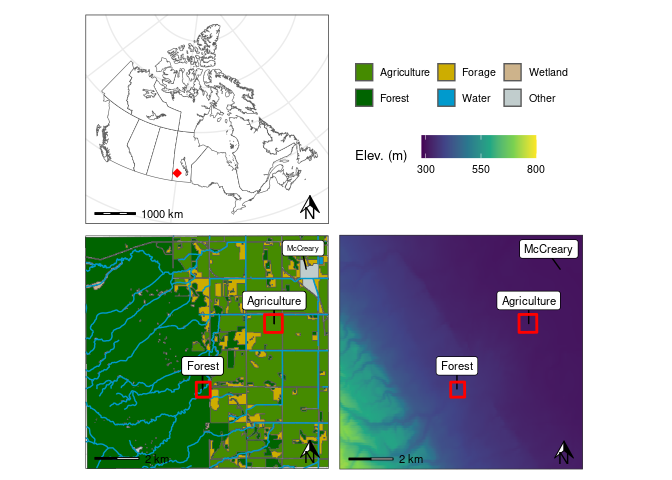
\includegraphics{index_files/figure-latex/notebooks-location_map-fig-location_map-output-2.png}

}

\caption{\label{fig-location_map}Map showing the location of the study
sites within Canada, and the regional land use and topography.}

\end{figure}%

\textsubscript{Source:
\href{https://alex-koiter.github.io/spatial-variability-soil-manuscript/notebooks/location_map.qmd.html\#cell-fig-location_map}{Research
Site Locations}}

\section{Results}\label{results}

\subsection{Univariate summary}\label{univariate-summary}

\begin{longtable}[]{@{}
  >{\centering\arraybackslash}p{(\columnwidth - 12\tabcolsep) * \real{0.1429}}
  >{\centering\arraybackslash}p{(\columnwidth - 12\tabcolsep) * \real{0.1429}}
  >{\centering\arraybackslash}p{(\columnwidth - 12\tabcolsep) * \real{0.1429}}
  >{\centering\arraybackslash}p{(\columnwidth - 12\tabcolsep) * \real{0.1429}}
  >{\centering\arraybackslash}p{(\columnwidth - 12\tabcolsep) * \real{0.1429}}
  >{\centering\arraybackslash}p{(\columnwidth - 12\tabcolsep) * \real{0.1429}}
  >{\centering\arraybackslash}p{(\columnwidth - 12\tabcolsep) * \real{0.1429}}@{}}

\caption{\label{tbl-univariate-summary}Summary statistics for for six
examples of for six examples of geochemical and colour soil properties,
specific surface area, and organic matter content for each site.}

\tabularnewline

\toprule\noalign{}
\begin{minipage}[b]{\linewidth}\centering
Element
\end{minipage} & \begin{minipage}[b]{\linewidth}\centering
Mean
\end{minipage} & \begin{minipage}[b]{\linewidth}\centering
SD
\end{minipage} & \begin{minipage}[b]{\linewidth}\centering
Max
\end{minipage} & \begin{minipage}[b]{\linewidth}\centering
Min
\end{minipage} & \begin{minipage}[b]{\linewidth}\centering
Skewness
\end{minipage} & \begin{minipage}[b]{\linewidth}\centering
CV
\end{minipage} \\
\midrule\noalign{}
\endhead
\bottomrule\noalign{}
\endlastfoot
\multicolumn{7}{@{}>{\centering\arraybackslash}p{(\columnwidth - 12\tabcolsep) * \real{1.0000} + 12\tabcolsep}@{}}{%
Forest} \\
\begin{minipage}[t]{\linewidth}\centering
Li
\end{minipage} & 6.47 & 0.90 & 8.60 & 4.30 & −0.02 & 13.89 \\
\begin{minipage}[t]{\linewidth}\centering
Nb
\end{minipage} & 0.37 & 0.06 & 0.56 & 0.17 & −0.68 & 17.10 \\
\begin{minipage}[t]{\linewidth}\centering
Zn
\end{minipage} & 109.55 & 53.27 & 318.00 & 42.00 & 1.43 & 48.62 \\
\begin{minipage}[t]{\linewidth}\centering
\emph{h}*
\end{minipage} & 1.13 & 0.05 & 1.23 & 1.06 & 0.34 & 4.13 \\
\begin{minipage}[t]{\linewidth}\centering
\emph{L}
\end{minipage} & 47.45 & 6.35 & 59.48 & 34.34 & −0.02 & 13.37 \\
\begin{minipage}[t]{\linewidth}\centering
\emph{v}*
\end{minipage} & 4.79 & 1.04 & 6.62 & 2.77 & 0.31 & 21.74 \\
\begin{minipage}[t]{\linewidth}\centering
SSA
\end{minipage} & 763.48 & 133.48 & 1,032.61 & 492.59 & −0.08 & 17.48 \\
\begin{minipage}[t]{\linewidth}\centering
Org
\end{minipage} & 11.55 & 5.99 & 26.99 & 1.37 & 0.37 & 51.89 \\
\multicolumn{7}{@{}>{\centering\arraybackslash}p{(\columnwidth - 12\tabcolsep) * \real{1.0000} + 12\tabcolsep}@{}}{%
Agriculture} \\
\begin{minipage}[t]{\linewidth}\centering
Ca
\end{minipage} & 4.00 & 2.19 & 8.78 & 0.95 & 0.28 & 54.66 \\
\begin{minipage}[t]{\linewidth}\centering
Mo
\end{minipage} & 0.93 & 0.41 & 2.35 & 0.47 & 1.18 & 43.95 \\
\begin{minipage}[t]{\linewidth}\centering
U
\end{minipage} & 1.48 & 0.19 & 1.94 & 1.20 & 0.59 & 12.64 \\
\begin{minipage}[t]{\linewidth}\centering
\emph{a}*
\end{minipage} & 3.38 & 0.32 & 4.15 & 2.59 & −0.03 & 9.53 \\
\begin{minipage}[t]{\linewidth}\centering
\emph{c}*
\end{minipage} & 9.47 & 1.02 & 11.32 & 7.17 & −0.19 & 10.74 \\
\begin{minipage}[t]{\linewidth}\centering
\emph{h}*
\end{minipage} & 1.20 & 0.01 & 1.23 & 1.18 & 0.19 & 1.12 \\
\begin{minipage}[t]{\linewidth}\centering
SSA
\end{minipage} & 1,853.02 & 187.32 & 2,195.72 & 1,458.53 & 0.00 &
10.11 \\
\begin{minipage}[t]{\linewidth}\centering
Org
\end{minipage} & 8.51 & 1.37 & 11.36 & 5.86 & 0.07 & 16.13 \\

\end{longtable}

\textsubscript{Source:
\href{https://alex-koiter.github.io/spatial-variability-soil-manuscript/notebooks/univariate_summary.qmd.html\#cell-tbl-univariate-summary}{Univariate
summary}}

\begin{longtable}[]{@{}
  >{\centering\arraybackslash}p{(\columnwidth - 12\tabcolsep) * \real{0.1429}}
  >{\centering\arraybackslash}p{(\columnwidth - 12\tabcolsep) * \real{0.1429}}
  >{\centering\arraybackslash}p{(\columnwidth - 12\tabcolsep) * \real{0.1429}}
  >{\centering\arraybackslash}p{(\columnwidth - 12\tabcolsep) * \real{0.1429}}
  >{\centering\arraybackslash}p{(\columnwidth - 12\tabcolsep) * \real{0.1429}}
  >{\centering\arraybackslash}p{(\columnwidth - 12\tabcolsep) * \real{0.1429}}
  >{\centering\arraybackslash}p{(\columnwidth - 12\tabcolsep) * \real{0.1429}}@{}}

\caption{\label{tbl-univariate2-summary}Summary statistics for the
interpoloated values (10m resolution) for six examples of geochemical
and colour soil properties, specific surface area, organic matter
content, and seven terrain attributes for each site.}

\tabularnewline

\toprule\noalign{}
\begin{minipage}[b]{\linewidth}\centering
Property
\end{minipage} & \begin{minipage}[b]{\linewidth}\centering
Mean
\end{minipage} & \begin{minipage}[b]{\linewidth}\centering
SD
\end{minipage} & \begin{minipage}[b]{\linewidth}\centering
Max
\end{minipage} & \begin{minipage}[b]{\linewidth}\centering
Min
\end{minipage} & \begin{minipage}[b]{\linewidth}\centering
Skewness
\end{minipage} & \begin{minipage}[b]{\linewidth}\centering
CV
\end{minipage} \\
\midrule\noalign{}
\endhead
\bottomrule\noalign{}
\endlastfoot
\multicolumn{7}{@{}>{\centering\arraybackslash}p{(\columnwidth - 12\tabcolsep) * \real{1.0000} + 12\tabcolsep}@{}}{%
Forest} \\
\begin{minipage}[t]{\linewidth}\centering
Li
\end{minipage} & 6.44 & 0.63 & 8.57 & 4.34 & −0.16 & 9.73 \\
\begin{minipage}[t]{\linewidth}\centering
Nb
\end{minipage} & 0.37 & 0.03 & 0.43 & 0.29 & −0.32 & 8.32 \\
\begin{minipage}[t]{\linewidth}\centering
Zn
\end{minipage} & 111.46 & 43.21 & 317.76 & 42.15 & 1.11 & 38.76 \\
\begin{minipage}[t]{\linewidth}\centering
\emph{h}*
\end{minipage} & 1.13 & 0.04 & 1.23 & 1.06 & 0.30 & 3.38 \\
\begin{minipage}[t]{\linewidth}\centering
\emph{L}
\end{minipage} & 47.25 & 4.72 & 59.48 & 34.38 & 0.10 & 9.98 \\
\begin{minipage}[t]{\linewidth}\centering
\emph{v}*
\end{minipage} & 4.78 & 0.73 & 6.62 & 2.77 & 0.28 & 15.28 \\
\begin{minipage}[t]{\linewidth}\centering
SSA
\end{minipage} & 760.40 & 120.58 & 1,102.95 & 483.70 & 0.12 & 15.86 \\
\begin{minipage}[t]{\linewidth}\centering
Org
\end{minipage} & 11.53 & 1.97 & 16.13 & 7.37 & −0.12 & 17.10 \\
\begin{minipage}[t]{\linewidth}\centering
Elevation
\end{minipage} & 369.28 & 3.34 & 377.24 & 358.29 & −0.21 & 0.90 \\
\begin{minipage}[t]{\linewidth}\centering
Rel. Slope Position
\end{minipage} & 0.22 & 0.26 & 1.00 & −0.12 & 1.55 & 116.75 \\
\begin{minipage}[t]{\linewidth}\centering
Vert. Dist. Channel
\end{minipage} & 0.47 & 0.57 & 4.90 & −0.67 & 2.75 & 122.69 \\
\begin{minipage}[t]{\linewidth}\centering
SAGA Wetness Index
\end{minipage} & 6.00 & 1.26 & 9.96 & 0.09 & −0.86 & 20.92 \\
\begin{minipage}[t]{\linewidth}\centering
Catchment Area
\end{minipage} & 565.06 & 5,109.73 & 209,263.22 & 0.67 & 17.83 &
904.28 \\
\begin{minipage}[t]{\linewidth}\centering
Profile Curvature
\end{minipage} & 0.00 & 0.03 & 0.45 & −0.47 & −0.34 & −15,245.25 \\
\begin{minipage}[t]{\linewidth}\centering
Plan Curvature
\end{minipage} & 0.00 & 0.01 & 0.30 & −0.26 & 0.56 & 3,382.34 \\
\multicolumn{7}{@{}>{\centering\arraybackslash}p{(\columnwidth - 12\tabcolsep) * \real{1.0000} + 12\tabcolsep}@{}}{%
Agriculture} \\
\begin{minipage}[t]{\linewidth}\centering
Ca
\end{minipage} & 4.10 & 2.09 & 9.11 & 1.03 & 0.09 & 51.01 \\
\begin{minipage}[t]{\linewidth}\centering
Mo
\end{minipage} & 0.89 & 0.31 & 1.96 & 0.51 & 0.76 & 35.03 \\
\begin{minipage}[t]{\linewidth}\centering
U
\end{minipage} & 1.46 & 0.14 & 1.81 & 1.24 & 0.25 & 9.24 \\
\begin{minipage}[t]{\linewidth}\centering
\emph{a}*
\end{minipage} & 3.34 & 0.22 & 3.93 & 2.77 & 0.03 & 6.60 \\
\begin{minipage}[t]{\linewidth}\centering
\emph{c}*
\end{minipage} & 9.35 & 0.76 & 11.08 & 7.39 & −0.16 & 8.17 \\
\begin{minipage}[t]{\linewidth}\centering
\emph{h}*
\end{minipage} & 1.20 & 0.01 & 1.23 & 1.18 & −0.13 & 0.72 \\
\begin{minipage}[t]{\linewidth}\centering
SSA
\end{minipage} & 1,867.79 & 129.71 & 2,056.35 & 1,579.16 & −0.43 &
6.94 \\
\begin{minipage}[t]{\linewidth}\centering
Org
\end{minipage} & 8.62 & 0.68 & 10.30 & 7.08 & 0.34 & 7.89 \\
\begin{minipage}[t]{\linewidth}\centering
Elevation
\end{minipage} & 309.92 & 0.59 & 311.82 & 309.01 & 0.62 & 0.19 \\
\begin{minipage}[t]{\linewidth}\centering
Rel. Slope Position
\end{minipage} & 0.72 & 0.34 & 28.79 & −33.19 & −3.62 & 47.84 \\
\begin{minipage}[t]{\linewidth}\centering
Vert. Dist. Channel
\end{minipage} & 0.06 & 0.04 & 0.33 & 0.00 & 1.07 & 73.73 \\
\begin{minipage}[t]{\linewidth}\centering
SAGA Wetness Index
\end{minipage} & 9.64 & 0.72 & 11.27 & 7.63 & −0.11 & 7.43 \\
\begin{minipage}[t]{\linewidth}\centering
Catchment Area
\end{minipage} & 475.21 & 1,884.43 & 41,848.99 & 1.05 & 10.24 &
396.55 \\
\begin{minipage}[t]{\linewidth}\centering
Profile Curvature
\end{minipage} & 0.00 & 0.00 & 0.00 & 0.00 & −0.15 & −5,332.23 \\
\begin{minipage}[t]{\linewidth}\centering
Plan Curvature
\end{minipage} & 0.00 & 0.00 & 0.00 & 0.00 & 0.23 & 27,643.82 \\

\end{longtable}

\textsubscript{Source:
\href{https://alex-koiter.github.io/spatial-variability-soil-manuscript/notebooks/univariate_summary.qmd.html\#cell-tbl-univariate2-summary}{Univariate
summary}}

\subsection{Spatial analysis}\label{spatial-analysis}

\begin{longtable}[]{@{}ccccccccc@{}}

\caption{\label{tbl-geochem-semivariogram}Geostatistical parameters of
the fitted semivariogram models for six examples of geochemical and
colour fingerprint properties for each site.}

\tabularnewline

\toprule\noalign{}
Property & Model{\textsuperscript{1}} & Nugget (Co) & Sill (Co) & Range
(m) & C/(C + Co) (\%) & Class{\textsuperscript{2}} & R2 & RMSE \\
\midrule\noalign{}
\endhead
\midrule\noalign{}
\multicolumn{9}{@{}c@{}}{%
{\textsuperscript{1}} Models are all isotropic.} \\
\multicolumn{9}{@{}c@{}}{%
{\textsuperscript{2}} S = strong spatial dependency (C/(C + Co) \%
\textgreater75); M = moderate spatial dependency (C/(C + Co) \% between
75 and 25).} \\
\bottomrule\noalign{}
\endlastfoot
\multicolumn{9}{@{}c@{}}{%
Agriculture} \\
Ca & Exp & 0 & 1.49 & 72.52 & 0 & S & 0.27 & 1.8 \\
\multicolumn{9}{@{}c@{}}{%
Forest} \\
Ca & Exp & 0 & 1.49 & 72.52 & 0 & S & 0.27 & 1.8 \\

\end{longtable}

\textsubscript{Source:
\href{https://alex-koiter.github.io/spatial-variability-soil-manuscript/notebooks/semivariogram.qmd.html\#cell-tbl-geochem-semivariogram}{Semivariograms}}

\begin{figure}[H]

\centering{

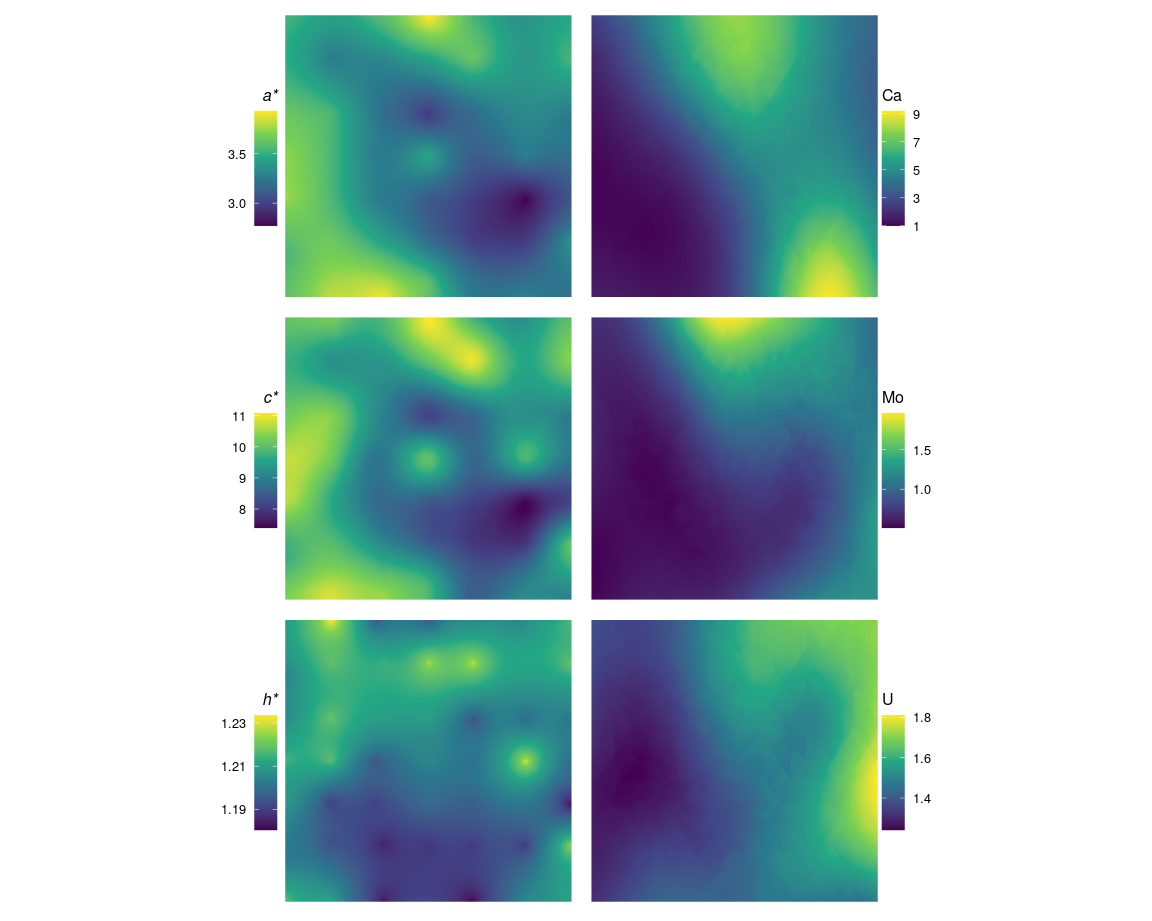
\includegraphics{index_files/figure-latex/notebooks-soil_property_maps-fig-ag_map-output-1.png}

}

\caption{\label{fig-ag_map}Kriged map of select colour (\emph{a*},
\emph{c*}, \emph{h*}) and geochemical (Ca, Mo, U) properties across the
agricultural site.}

\end{figure}%

\textsubscript{Source:
\href{https://alex-koiter.github.io/spatial-variability-soil-manuscript/notebooks/soil_property_maps.qmd.html\#cell-fig-ag_map}{Soil
property mapping}}

\begin{figure}[H]

\centering{

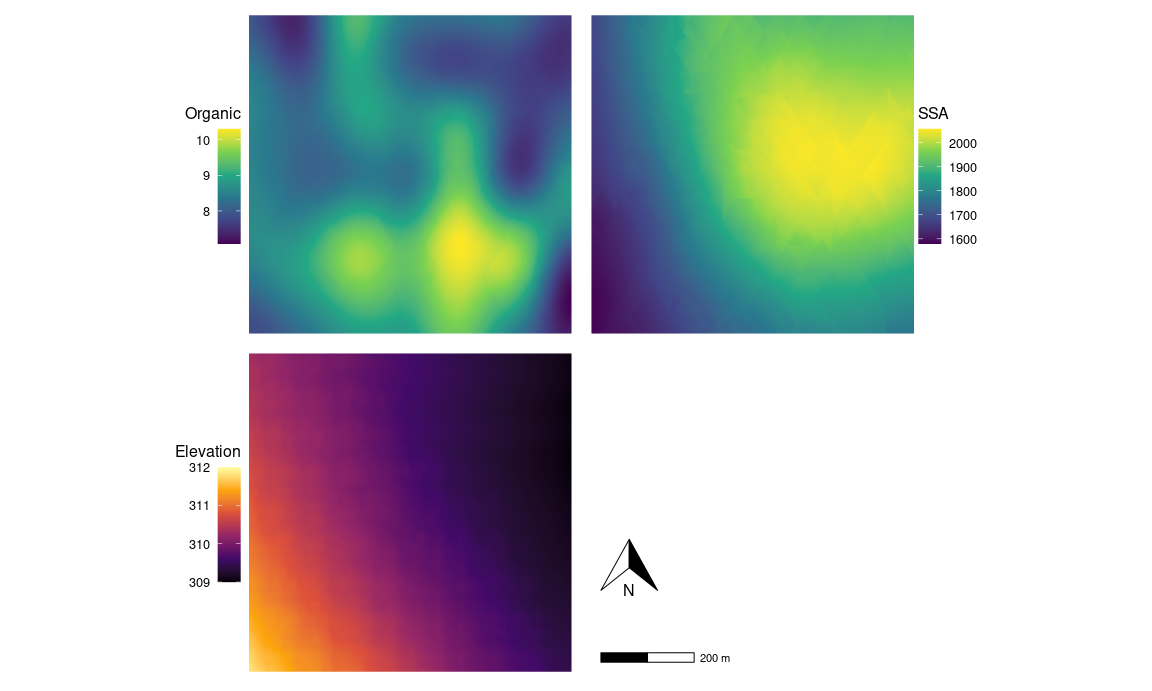
\includegraphics{index_files/figure-latex/notebooks-soil_property_maps-fig-ag_map2-output-1.png}

}

\caption{\label{fig-ag_map2}Kriged map of organic matter content (\%),
specific surface area (m2 kg-1), and elevation (m) across the
agricultural site.}

\end{figure}%

\textsubscript{Source:
\href{https://alex-koiter.github.io/spatial-variability-soil-manuscript/notebooks/soil_property_maps.qmd.html\#cell-fig-ag_map2}{Soil
property mapping}}

\begin{figure}[H]

\centering{

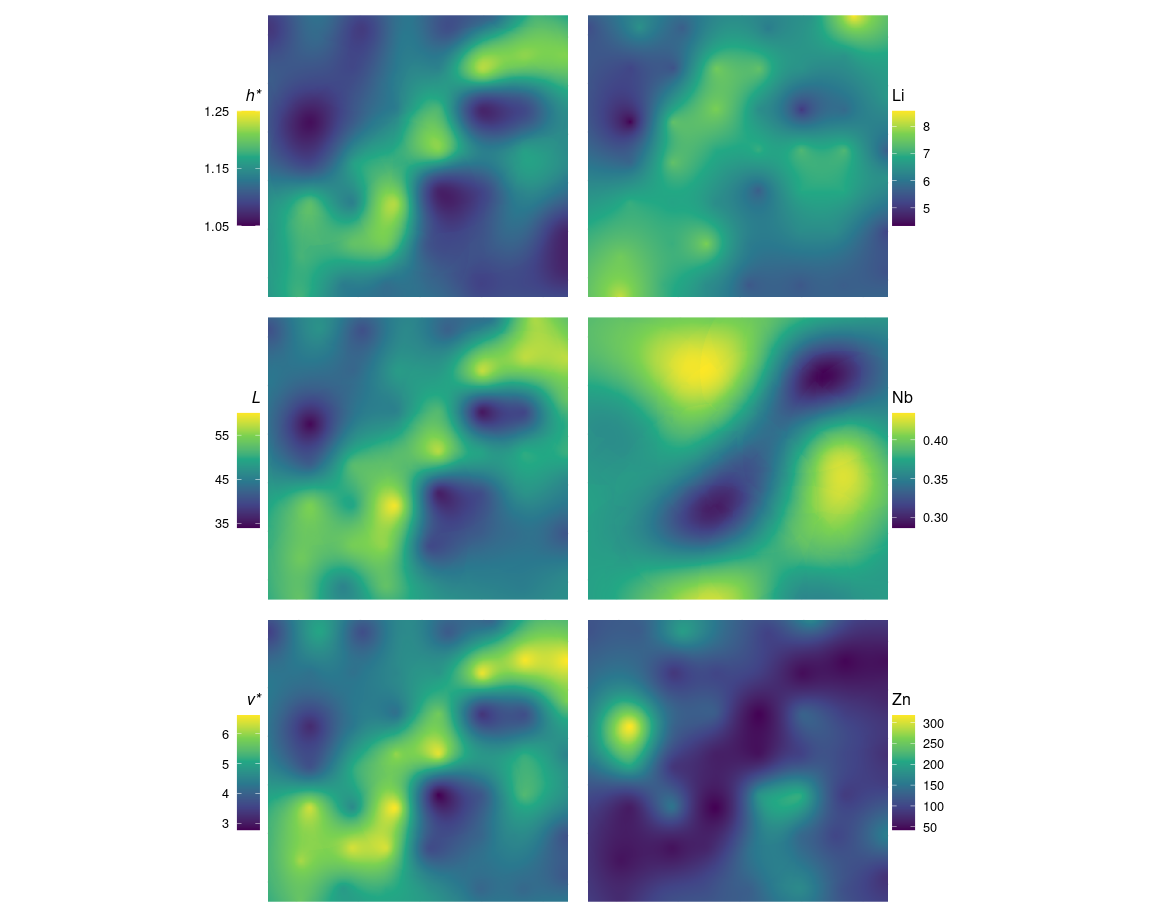
\includegraphics{index_files/figure-latex/notebooks-soil_property_maps-fig-forest_map-output-1.png}

}

\caption{\label{fig-forest_map}Kriged map of select colour (\emph{h*},
\emph{c*}, \emph{v*}) and geochemical (Li, Nb, Zn) properties across the
forested site.}

\end{figure}%

\textsubscript{Source:
\href{https://alex-koiter.github.io/spatial-variability-soil-manuscript/notebooks/soil_property_maps.qmd.html\#cell-fig-forest_map}{Soil
property mapping}}

\begin{figure}[H]

\centering{

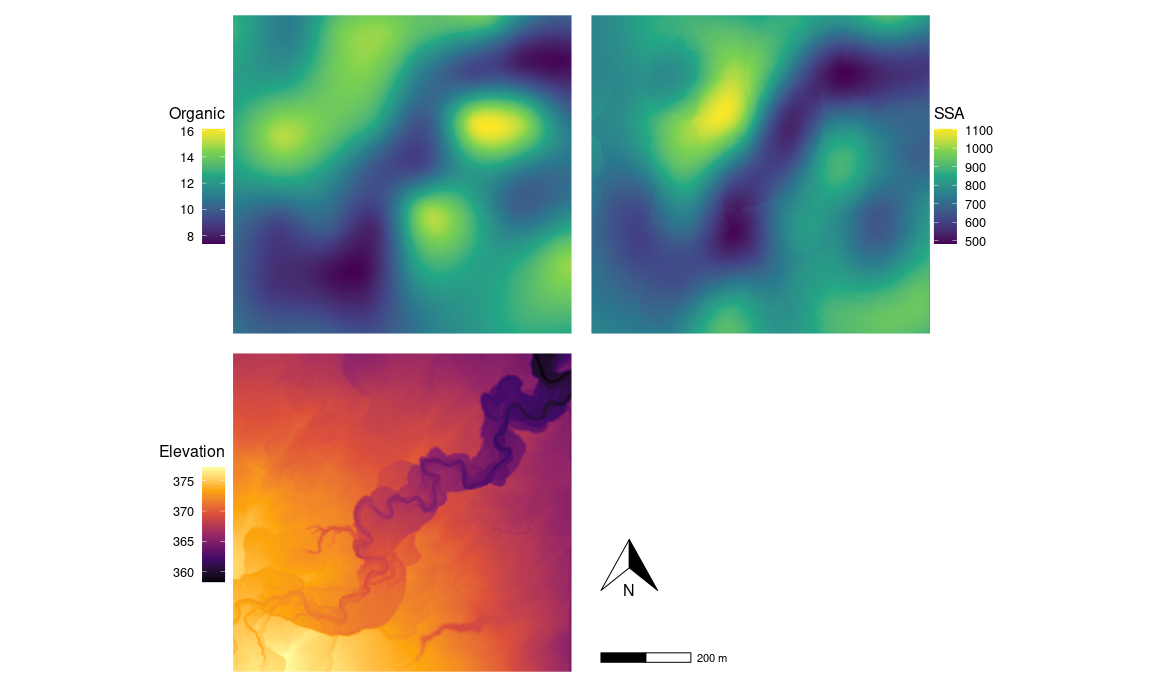
\includegraphics{index_files/figure-latex/notebooks-soil_property_maps-fig-forest_map2-output-1.png}

}

\caption{\label{fig-forest_map2}Kriged map of organic matter content
(\%), specific surface area (m2 kg-1), and elevation (m) across the
forested site.}

\end{figure}%

\textsubscript{Source:
\href{https://alex-koiter.github.io/spatial-variability-soil-manuscript/notebooks/soil_property_maps.qmd.html\#cell-fig-forest_map2}{Soil
property mapping}}

\begin{figure}[H]

\centering{

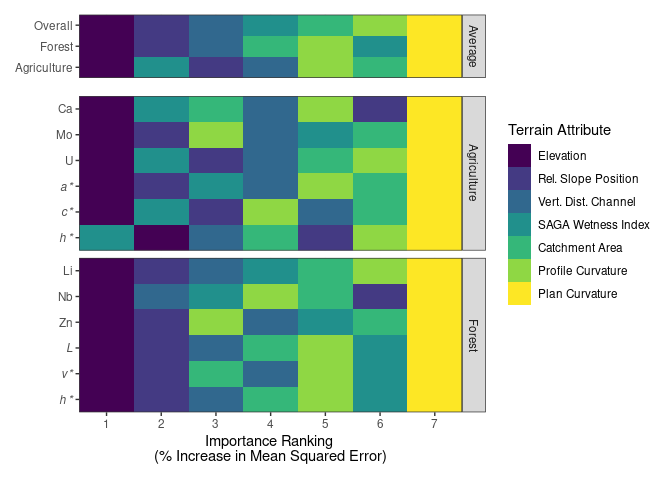
\includegraphics{index_files/figure-latex/notebooks-RF_results-fig-rf-results-output-1.png}

}

\caption{\label{fig-rf-results}Heat map of the Random Forest regresssion
results showing the ranking of the importance of terrain attributes
(based on \% increase in Mean Squared Error) in explaining the spatial
variabilty of selected colour and geochemical properties within the
agricultural and forested sites. Top panel shows an average ranking for
each site and across both sites.}

\end{figure}%

\textsubscript{Source:
\href{https://alex-koiter.github.io/spatial-variability-soil-manuscript/notebooks/RF_results.qmd.html\#cell-fig-RF-results}{Random
Forest results}}

\section*{References}\label{references}
\addcontentsline{toc}{section}{References}

\renewcommand{\bibsection}{}
\bibliography{references.bib}

\section*{Supplemental materials}\label{supplemental-materials}
\addcontentsline{toc}{section}{Supplemental materials}

\phantomsection\label{ssuppfig-geo_summary}
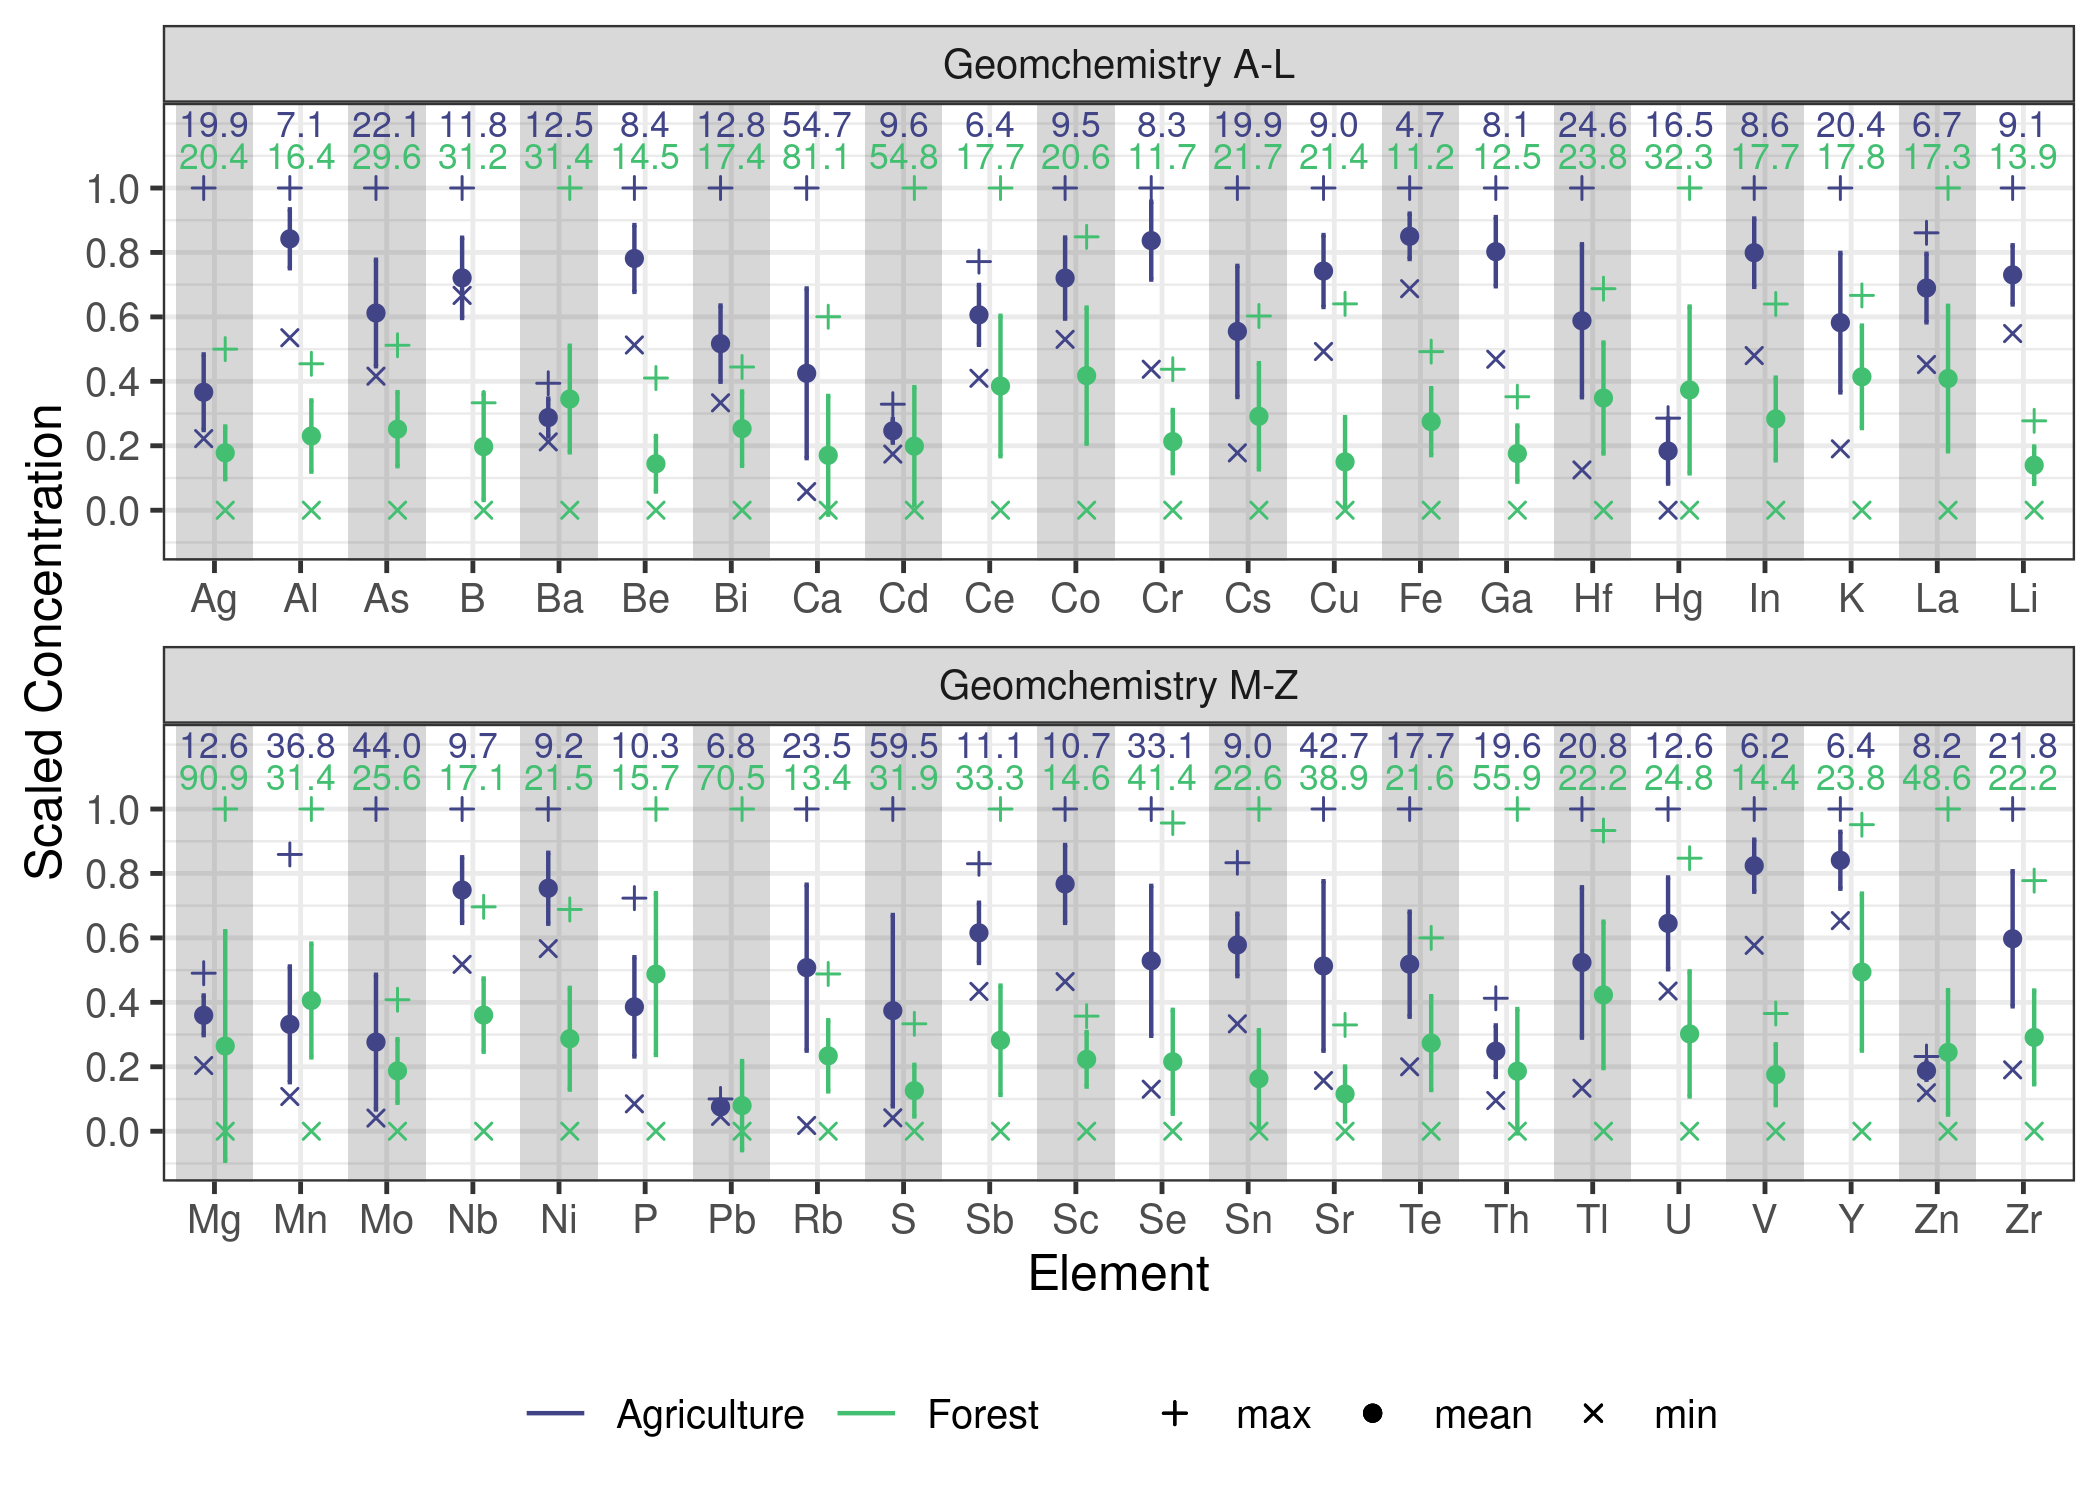
\includegraphics{images/geo_summary.png}

Summary statistics of all measured geochemical soil properties at both
sites. Error bars represent 1SD and the numeric values indicate the CV.

\phantomsection\label{ssuppfig-colour_summary}
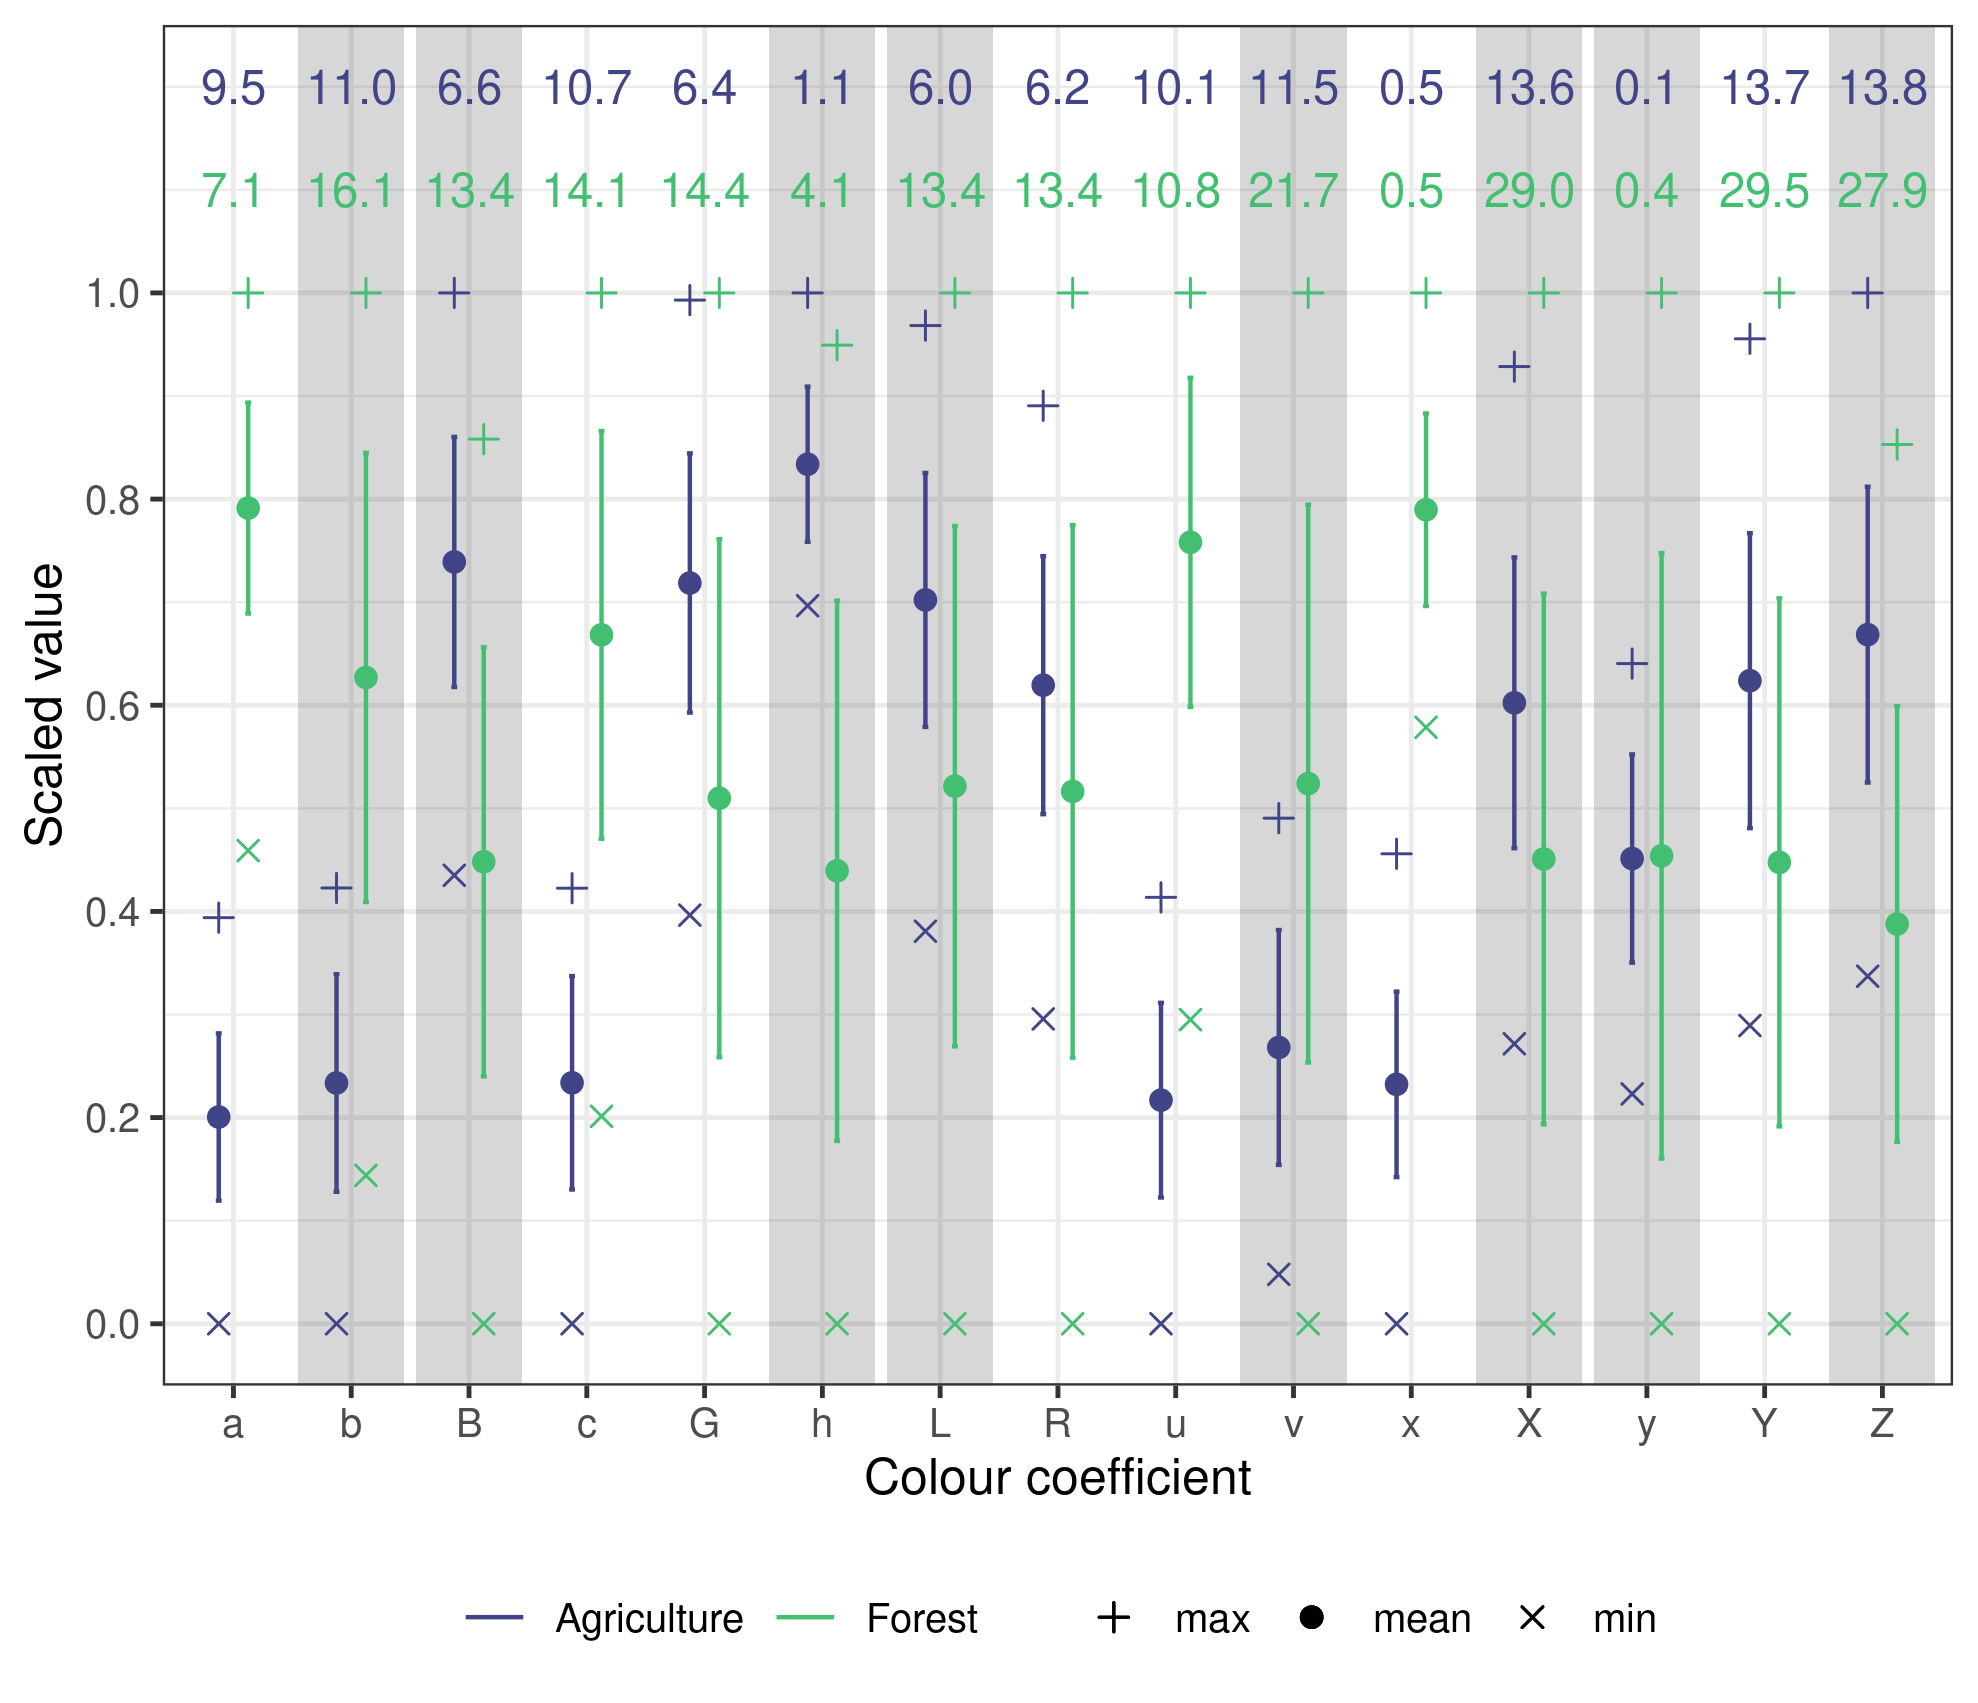
\includegraphics{images/colour_summary.png}

Summary statistics of all measured colour soil properties at both sites.
Error bars represent 1SD and the numeric values indicate the CV.




\end{document}
